% Scripted test round for the feedback reader. One sentence per line.
% Each target sentence ends with a comment naming its id, the word to click and the expected note (see eval.py).
% kind=general: a general remark (no location). kind=absent: must NOT appear (discarded or deleted).
% Build with `latexmk -pdf -synctex=1 targets.tex`, open the PDF in the reader, do the round, then score it:
% python3 tests/eval.py tests/targets.tex [<round dir>]
\documentclass[11pt,a4paper]{article}
\usepackage[margin=2.5cm]{geometry}
\usepackage{amsmath}
\usepackage[version=4]{mhchem}
\usepackage{siunitx}
\usepackage{tikz}
\usepackage{xcolor}
\definecolor{instr}{HTML}{1F5FAD}
\newcommand{\instr}[2]{\par\smallskip\noindent\colorbox{instr!10}{\parbox{\dimexpr\linewidth-2\fboxsep}{\small\color{instr}\textbf{#1}\quad #2}}\par\smallskip}
\setlength{\parindent}{0pt}
\setlength{\parskip}{4pt}

\begin{document}

\section*{Feedback reader test round}

\instr{How}{Do the targets in order. Speak normally after each click. Save with Enter unless told otherwise. When all are done, press \textbf{Finish round}.}

Halide perovskites are soft, anharmonic crystals whose structure fluctuates strongly at room temperature. % TARGET id=T1 word=anharmonic expect="Shorten this sentence."
\instr{T1}{Click on \textbf{anharmonic}. Say: ``Shorten this sentence.''}

The relative stability of competing phases depends on how these fluctuations are treated in the calculations that are performed for each candidate structure.
Static calculations at \SI{0}{\kelvin} can therefore misrepresent which phase is stable. % TARGET id=T2 word=Static expect="Cut this sentence."
\instr{T2}{This sentence starts in the middle of a printed line. Click on its first word, \textbf{Static}. Say: ``Cut this sentence.''}

The machine-learning interatomic potential was trained on configurations of \ce{CsPbI3} sampled from molecular dynamics. % TARGET id=T3 word=trained expect="Change CsPbI3 to CsPbBr3 in this sentence."
\instr{T3}{Click on \textbf{trained}. Say: ``Change CsPbI3 to CsPbBr3 in this sentence.'' (tests the dictionary)}

All production runs, which together amounted to several hundred nanoseconds of simulation time across five temperatures and three system sizes, were carried out on the Isambard supercomputer using LAMMPS with the MACE potential loaded through its plugin interface. % TARGET id=T4 word=Isambard expect="Say these runs used ARCHER2, not Isambard."
\instr{T4}{A long sentence over several printed lines. Click on \textbf{Isambard}, on a later line. Say: ``Say these runs used ARCHER2, not Isambard.''}

We utilise the same potential for every polytype. % TARGET id=T5 word=utilise expect="Replace utilise with use."
\instr{T5}{Typing only. Press \textbf{M} to turn the mic off, click on \textbf{utilise}, type: \texttt{Replace utilise with use.}, press Enter, then press \textbf{M} again.}

\begin{figure}[h]
	\centering
	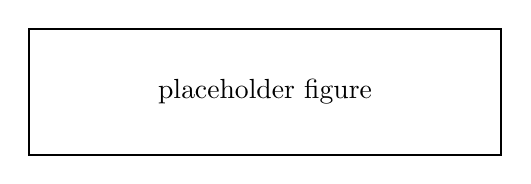
\begin{tikzpicture}\draw[thick] (0,0) rectangle (6,1.6); \node at (3,0.8) {placeholder figure};\end{tikzpicture}
	\caption{Free energy of the hexagonal polytypes relative to the cubic phase, from thermodynamic integration.} % TARGET id=T6 word=thermodynamic expect="Add the temperature range to the caption."
\end{figure}
\instr{T6}{Click on \textbf{thermodynamic} in the caption above. Say: ``Add the temperature range to the caption.''}

The free energy follows from thermodynamic integration between the harmonic and the anharmonic system,
\begin{equation}
	F(T) = E_0 - T S_\text{vib}(T) + \int_0^1 \langle U_1 - U_0 \rangle_\lambda \, \mathrm{d}\lambda . % TARGET id=T7 word= expect="Define every symbol in this equation."
\end{equation}
\instr{T7}{Click on the integral sign in the equation. Say: ``Define every symbol in this equation.''}

\instr{T8}{General remark. Press \textbf{G} (or the General remark button). Say: ``Use British spelling throughout.''} % TARGET id=T8 kind=general expect="Use British spelling throughout."

The electron-phonon coupling of these modes is quantified through Huang-Rhys factors. % TARGET id=T9 word=Huang-Rhys expect="Add a citation here."
\instr{T9}{Click on \textbf{Huang-Rhys}. Say: ``Add a citation here.'' Then save by clicking \textbf{the same pin again}, not Enter.}

This sentence exists only to be commented on and then deleted. % TARGET id=T10 kind=absent word=deleted expect="This note should be deleted."
\instr{T10}{Click on \textbf{deleted}. Say: ``This note should be deleted.'' Save it. Then press \textbf{Open} on it in the list and \textbf{Delete}.}

This sentence exists only to test discarding. % TARGET id=T11 kind=absent word=discarding expect="Discard me."
\instr{T11}{Click on \textbf{discarding}. Say: ``Discard me.'' Then press \textbf{Esc} instead of saving.}

\end{document}
